\documentclass{standalone}
\usepackage{tikz}
\usetikzlibrary{patterns, positioning}


\begin{document}
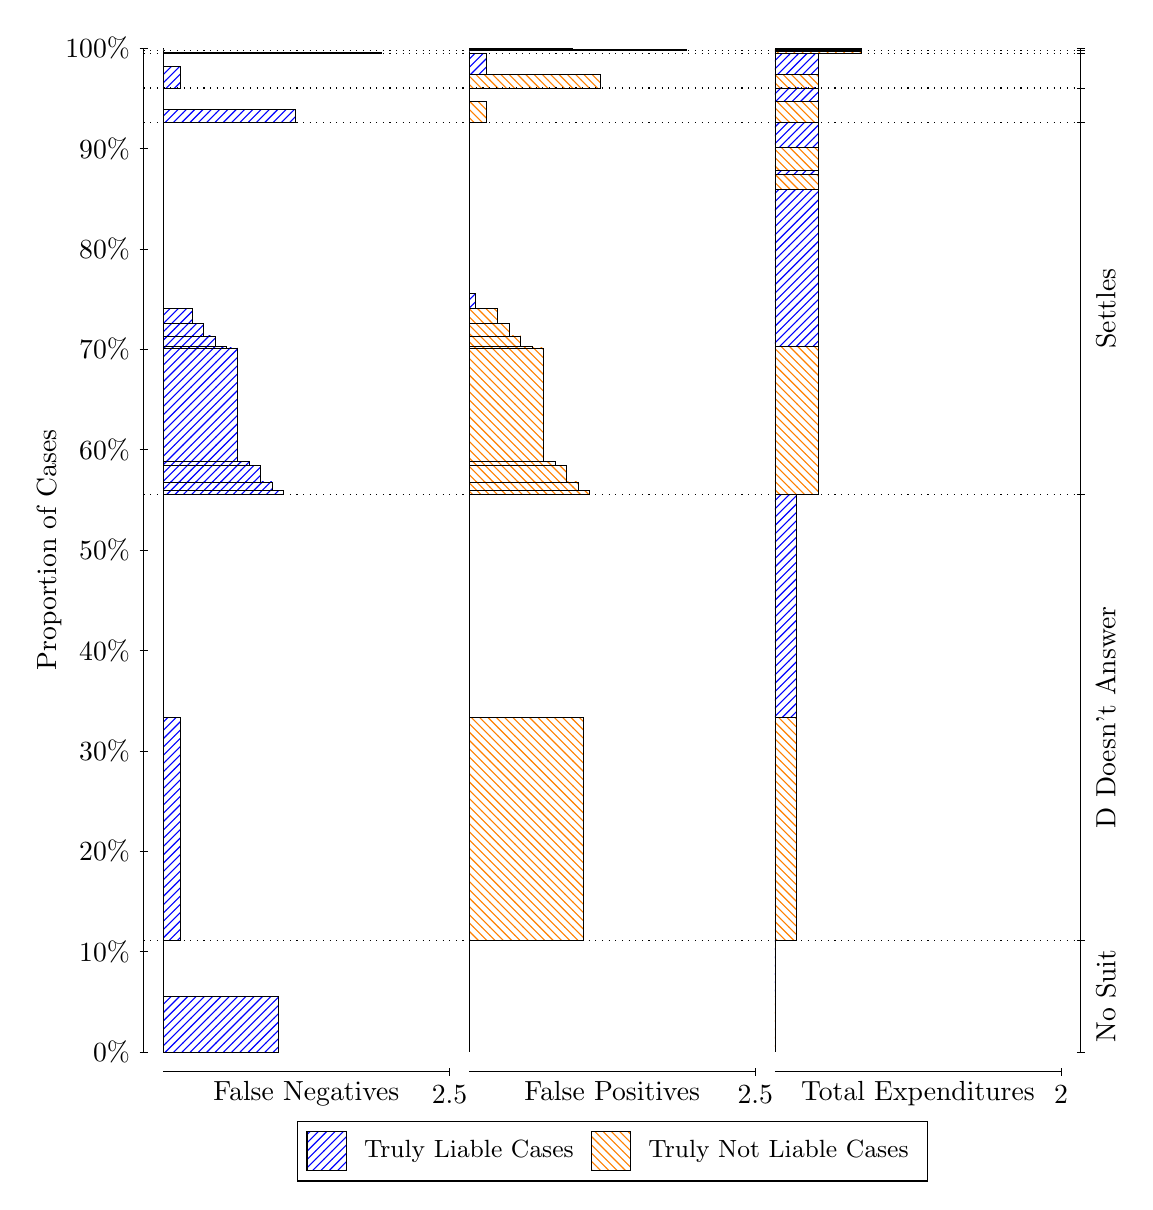
\begin{tikzpicture}
\draw[black, very thin] (1.5,1.75) -- (1.5,14.5);
\node[rotate=90, text=black, anchor=center] at (0.3, 8.125) {Proportion of Cases};
\draw[black, very thin] (1.45,1.75) -- (1.55,1.75);
\node[text=black, anchor=east] at (1.45, 1.75) {0\%};
\draw[black, very thin] (1.45,3.025) -- (1.55,3.025);
\node[text=black, anchor=east] at (1.45, 3.025) {10\%};
\draw[black, very thin] (1.45,4.3) -- (1.55,4.3);
\node[text=black, anchor=east] at (1.45, 4.3) {20\%};
\draw[black, very thin] (1.45,5.575) -- (1.55,5.575);
\node[text=black, anchor=east] at (1.45, 5.575) {30\%};
\draw[black, very thin] (1.45,6.85) -- (1.55,6.85);
\node[text=black, anchor=east] at (1.45, 6.85) {40\%};
\draw[black, very thin] (1.45,8.125) -- (1.55,8.125);
\node[text=black, anchor=east] at (1.45, 8.125) {50\%};
\draw[black, very thin] (1.45,9.4) -- (1.55,9.4);
\node[text=black, anchor=east] at (1.45, 9.4) {60\%};
\draw[black, very thin] (1.45,10.675) -- (1.55,10.675);
\node[text=black, anchor=east] at (1.45, 10.675) {70\%};
\draw[black, very thin] (1.45,11.95) -- (1.55,11.95);
\node[text=black, anchor=east] at (1.45, 11.95) {80\%};
\draw[black, very thin] (1.45,13.225) -- (1.55,13.225);
\node[text=black, anchor=east] at (1.45, 13.225) {90\%};
\draw[black, very thin] (1.45,14.5) -- (1.55,14.5);
\node[text=black, anchor=east] at (1.45, 14.5) {100\%};

\draw[black, very thin] (13.4,1.75) -- (13.4,14.5);
\draw[black, very thin] (13.35,1.75) -- (13.45,1.75);
\node[anchor=west] at (13.35, 1.75) {};
\draw[black, very thin] (13.35,3.1667) -- (13.45,3.1667);
\node[anchor=west] at (13.35, 3.1667) {};
\draw[black, very thin] (13.35,8.8333) -- (13.45,8.8333);
\node[anchor=west] at (13.35, 8.8333) {};
\draw[black, very thin] (13.35,13.551) -- (13.45,13.551);
\node[anchor=west] at (13.35, 13.551) {};
\draw[black, very thin] (13.35,13.993) -- (13.45,13.993);
\node[anchor=west] at (13.35, 13.993) {};
\draw[black, very thin] (13.35,14.436) -- (13.45,14.436);
\node[anchor=west] at (13.35, 14.436) {};
\draw[black, very thin] (13.35,14.468) -- (13.45,14.468);
\node[anchor=west] at (13.35, 14.468) {};
\draw[black, very thin] (13.35,14.5) -- (13.45,14.5);
\node[anchor=west] at (13.35, 14.5) {};

\draw[black, very thin, pattern color=blue, pattern=north east lines] (1.75,1.75) rectangle (3.2033,2.4583);
\draw[black, very thin, pattern color=orange, pattern=north west lines] (1.75,2.4583) rectangle (1.75,3.1667);
\draw[black, very thin, pattern color=blue, pattern=north east lines] (1.75,3.1667) rectangle (1.968,6);
\draw[black, very thin, pattern color=orange, pattern=north west lines] (1.75,6) rectangle (1.75,8.8333);
\draw[black, very thin, pattern color=blue, pattern=north east lines] (1.75,8.8333) rectangle (3.276,8.8853);
\draw[black, very thin, pattern color=blue, pattern=north east lines] (1.75,8.8853) rectangle (3.1307,8.9905);
\draw[black, very thin, pattern color=blue, pattern=north east lines] (1.75,8.9905) rectangle (2.9853,9.2006);
\draw[black, very thin, pattern color=blue, pattern=north east lines] (1.75,9.2006) rectangle (2.84,9.2494);
\draw[black, very thin, pattern color=blue, pattern=north east lines] (1.75,9.2494) rectangle (2.6947,10.693);
\draw[black, very thin, pattern color=blue, pattern=north east lines] (1.75,10.693) rectangle (2.5493,10.71);
\draw[black, very thin, pattern color=blue, pattern=north east lines] (1.75,10.71) rectangle (2.404,10.844);
\draw[black, very thin, pattern color=blue, pattern=north east lines] (1.75,10.844) rectangle (2.2587,11.003);
\draw[black, very thin, pattern color=blue, pattern=north east lines] (1.75,11.003) rectangle (2.1133,11.192);
\draw[black, very thin, pattern color=orange, pattern=north west lines] (1.75,11.192) rectangle (1.75,13.551);
\draw[black, very thin, pattern color=blue, pattern=north east lines] (1.75,13.551) rectangle (3.4213,13.725);
\draw[black, very thin, pattern color=orange, pattern=north west lines] (1.75,13.725) rectangle (1.75,13.993);
\draw[black, very thin, pattern color=blue, pattern=north east lines] (1.75,13.993) rectangle (1.968,14.262);
\draw[black, very thin, pattern color=orange, pattern=north west lines] (1.75,14.262) rectangle (1.75,14.436);
\draw[black, very thin, pattern color=blue, pattern=north east lines] (1.75,14.436) rectangle (4.5113,14.448);
\draw[black, very thin, pattern color=orange, pattern=north west lines] (1.75,14.448) rectangle (1.75,14.468);
\draw[black, very thin, pattern color=orange, pattern=north west lines] (1.75,14.468) rectangle (1.75,14.48);
\draw[black, very thin, pattern color=blue, pattern=north east lines] (1.75,14.48) rectangle (1.75,14.5);
\draw[black, very thin, pattern color=orange, pattern=north west lines] (5.6333,1.75) rectangle (5.6333,2.4583);
\draw[black, very thin, pattern color=blue, pattern=north east lines] (5.6333,2.4583) rectangle (5.6333,3.1667);
\draw[black, very thin, pattern color=orange, pattern=north west lines] (5.6333,3.1667) rectangle (7.0867,6);
\draw[black, very thin, pattern color=blue, pattern=north east lines] (5.6333,6) rectangle (5.6333,8.8333);
\draw[black, very thin, pattern color=orange, pattern=north west lines] (5.6333,8.8333) rectangle (7.1593,8.8853);
\draw[black, very thin, pattern color=orange, pattern=north west lines] (5.6333,8.8853) rectangle (7.014,8.9906);
\draw[black, very thin, pattern color=orange, pattern=north west lines] (5.6333,8.9906) rectangle (6.8687,9.2006);
\draw[black, very thin, pattern color=orange, pattern=north west lines] (5.6333,9.2006) rectangle (6.7233,9.2494);
\draw[black, very thin, pattern color=orange, pattern=north west lines] (5.6333,9.2494) rectangle (6.578,10.693);
\draw[black, very thin, pattern color=orange, pattern=north west lines] (5.6333,10.693) rectangle (6.4327,10.71);
\draw[black, very thin, pattern color=orange, pattern=north west lines] (5.6333,10.71) rectangle (6.2873,10.844);
\draw[black, very thin, pattern color=orange, pattern=north west lines] (5.6333,10.844) rectangle (6.142,11.002);
\draw[black, very thin, pattern color=orange, pattern=north west lines] (5.6333,11.002) rectangle (5.9967,11.192);
\draw[black, very thin, pattern color=blue, pattern=north east lines] (5.6333,11.192) rectangle (5.706,11.382);
\draw[black, very thin, pattern color=blue, pattern=north east lines] (5.6333,11.382) rectangle (5.6333,13.551);
\draw[black, very thin, pattern color=orange, pattern=north west lines] (5.6333,13.551) rectangle (5.8513,13.82);
\draw[black, very thin, pattern color=blue, pattern=north east lines] (5.6333,13.82) rectangle (5.6333,13.993);
\draw[black, very thin, pattern color=orange, pattern=north west lines] (5.6333,13.993) rectangle (7.3047,14.167);
\draw[black, very thin, pattern color=blue, pattern=north east lines] (5.6333,14.167) rectangle (5.8513,14.436);
\draw[black, very thin, pattern color=orange, pattern=north west lines] (5.6333,14.436) rectangle (5.6333,14.456);
\draw[black, very thin, pattern color=blue, pattern=north east lines] (5.6333,14.456) rectangle (5.6333,14.468);
\draw[black, very thin, pattern color=orange, pattern=north west lines] (5.6333,14.468) rectangle (8.3947,14.48);
\draw[black, very thin, pattern color=blue, pattern=north east lines] (5.6333,14.48) rectangle (6.9413,14.5);
\draw[black, very thin, pattern color=orange, pattern=north west lines] (9.5167,1.75) rectangle (9.5167,2.4583);
\draw[black, very thin, pattern color=blue, pattern=north east lines] (9.5167,2.4583) rectangle (9.5167,3.1667);
\draw[black, very thin, pattern color=orange, pattern=north west lines] (9.5167,3.1667) rectangle (9.7892,6);
\draw[black, very thin, pattern color=blue, pattern=north east lines] (9.5167,6) rectangle (9.7892,8.8333);
\draw[black, very thin, pattern color=orange, pattern=north west lines] (9.5167,8.8333) rectangle (10.062,10.71);
\draw[black, very thin, pattern color=blue, pattern=north east lines] (9.5167,10.71) rectangle (10.062,12.701);
\draw[black, very thin, pattern color=orange, pattern=north west lines] (9.5167,12.701) rectangle (10.062,12.891);
\draw[black, very thin, pattern color=blue, pattern=north east lines] (9.5167,12.891) rectangle (10.062,12.943);
\draw[black, very thin, pattern color=orange, pattern=north west lines] (9.5167,12.943) rectangle (10.062,13.236);
\draw[black, very thin, pattern color=blue, pattern=north east lines] (9.5167,13.236) rectangle (10.062,13.551);
\draw[black, very thin, pattern color=orange, pattern=north west lines] (9.5167,13.551) rectangle (10.062,13.82);
\draw[black, very thin, pattern color=blue, pattern=north east lines] (9.5167,13.82) rectangle (10.062,13.993);
\draw[black, very thin, pattern color=orange, pattern=north west lines] (9.5167,13.993) rectangle (10.062,14.167);
\draw[black, very thin, pattern color=blue, pattern=north east lines] (9.5167,14.167) rectangle (10.062,14.436);
\draw[black, very thin, pattern color=orange, pattern=north west lines] (9.5167,14.436) rectangle (10.607,14.456);
\draw[black, very thin, pattern color=blue, pattern=north east lines] (9.5167,14.456) rectangle (10.607,14.468);
\draw[black, very thin, pattern color=orange, pattern=north west lines] (9.5167,14.468) rectangle (10.607,14.48);
\draw[black, very thin, pattern color=blue, pattern=north east lines] (9.5167,14.48) rectangle (10.607,14.5);
\draw[black, dotted] (1.5,3.1667) -- (13.4,3.1667);
\draw[black, dotted] (1.5,8.8333) -- (13.4,8.8333);
\draw[black, dotted] (1.5,13.551) -- (13.4,13.551);
\draw[black, dotted] (1.5,13.993) -- (13.4,13.993);
\draw[black, dotted] (1.5,14.436) -- (13.4,14.436);
\draw[black, dotted] (1.5,14.468) -- (13.4,14.468);
\draw[black, very thin] (1.75,1.5) -- (5.3833,1.5);
\node[text=black, anchor=north] at (3.5667, 1.5) {False Negatives};
\draw[black, very thin] (5.3833,1.45) -- (5.3833,1.55);
\node[text=black, anchor=north] at (5.3833, 1.45) {2.5};

\draw[black, very thin] (5.6333,1.5) -- (9.2667,1.5);
\node[text=black, anchor=north] at (7.45, 1.5) {False Positives};
\draw[black, very thin] (9.2667,1.45) -- (9.2667,1.55);
\node[text=black, anchor=north] at (9.2667, 1.45) {2.5};

\draw[black, very thin] (9.5167,1.5) -- (13.15,1.5);
\node[text=black, anchor=north] at (11.333, 1.5) {Total Expenditures};
\draw[black, very thin] (13.15,1.45) -- (13.15,1.55);
\node[text=black, anchor=north] at (13.15, 1.45) {2};

\node[text=black, centered, rotate=90] at (13.72, 2.4583) {No Suit};
\node[text=black, centered, rotate=90] at (13.72, 6) {D Doesn't Answer};
\node[text=black, centered, rotate=90] at (13.72, 11.192) {Settles};





\draw (7.449999999999999,1.5) node[draw=none] (baseCoordinate) {};
\begin{scope}[align=center]
        \matrix[scale=0.5, draw=black, below=0.5cm of baseCoordinate, nodes={draw}, column sep=0.1cm]{
            \node[rectangle, draw, minimum width=0.5cm, minimum height=0.5cm, pattern color=blue, pattern=north east lines] {}; &
            \node[draw=none, font=\small, text=black] (B) {Truly Liable Cases}; &
            \node[rectangle, draw, minimum width=0.5cm, minimum height=0.5cm, pattern color=orange, pattern=north west lines] {}; &
            \node[draw=none, font=\small, text=black] (B) {Truly Not Liable Cases}; \\
            };
\end{scope}

\end{tikzpicture}
\end{document}